\appendix
\Huge{\textbf{Appendices}}

\section{Augmented Images}\label{apx:augmentedImages}

\begin{figure}[h]
    \centering
    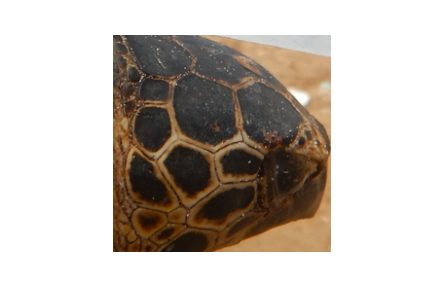
\includegraphics{images/turtles/base.png}
    \caption{Non-augmented image.}
    \label{fig:turtleBase}
\end{figure}

\begin{figure}[h!]
    \centering
    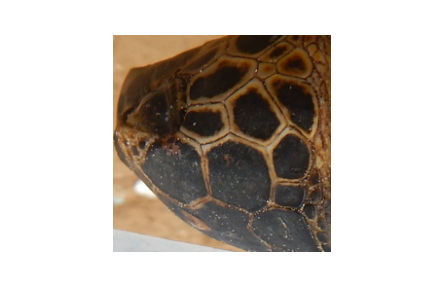
\includegraphics{images/turtles/rotated.png}
    \caption{Image rotated by 180 degrees.}
    \label{fig:turtleRotated}
\end{figure}

\begin{figure}[h!]
    \centering
    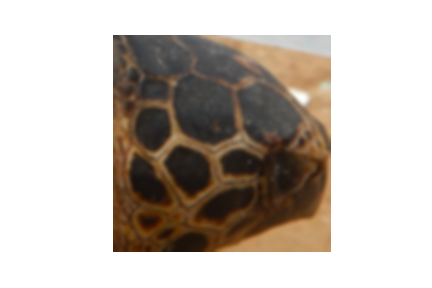
\includegraphics{images/turtles/gaussian.png}
    \caption{Image with Gauss-filter applied.}
    \label{fig:turtleGauss}
\end{figure}

\begin{figure}[h]
    \centering
    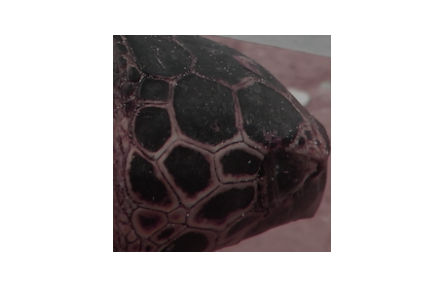
\includegraphics{images/turtles/hsv.png}
    \caption{Image with randomly changed HSV values.}
    \label{fig:turtleHSV}
\end{figure}

\begin{figure}[h]
    \centering
    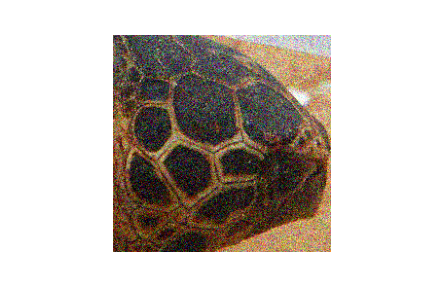
\includegraphics{images/turtles/noise.png}
    \caption{Image with added noise.}
    \label{fig:turtleNoise}
\end{figure}

\clearpage

\section{Dataset}\label{apx:minImages}
\begin{table}[h]
    \begin{tabular}{|l|c|c|c|c|c|c|c|c|}
    \hline
    \textbf{Min number images}                 & 8    & 9    & 10   & 11   & 12   & 13   & 14   & 15   \\ \hline
    \textbf{Images in dataset}               & 5846 & 5638 & 4990 & 4690 & 4338 & 3846 & 3560 & 3392 \\ \hline
    \textbf{Images per turtle (median)} & 12   & 12   & 14   & 15   & 16   & 18   & 21   & 22   \\ \hline
    \end{tabular}
    \caption[]{Dataset size in relation to number of images per turtle.}
    \label{tab:minImages}
\end{table}